% ==========================================
\section{Architettura software proposta}
% ==========================================

\subsection{Panoramica Architetturale}

% Per l'implementazione del sistema è stata scelta un'infrastruttura basata sullo stile \textbf{Client-Server}, strutturata internamente secondo il pattern architetturale \textbf{MVC (Model-View-Controller)} e integrata con il design pattern \textbf{Repository} per il disaccoppiamento dei dati.

% L'adozione del paradigma \textbf{Client-Server} è dettata dalla necessità di garantire una netta \textbf{separazione tra l'utente finale e i dati con cui questo interagisce}, i quali, per la natura stessa dell'applicazione, devono essere centralizzati e protetti.

% A livello applicativo, la logica è organizzata tramite il pattern \textbf{MVC}, il quale suddivide il sistema in tre sottosistemi principali:
% \begin{itemize}[itemsep=-6pt]
%     \item \textbf{Model subsystem:} responsabile di mantenere la conoscenza del dominio, gestisce la persistenza, l'integrità e la distribuzione dei dati.
%     \item \textbf{View subsystem:} responsabile di esibire gli elementi del dominio all'utente, costituisce l'interfaccia grafica attraverso la quale i dati vengono visualizzati.
%     \item \textbf{Controller subsystem:} responsabile di gestire la sequenza delle interazioni, definisce i metodi con cui l'utente interroga il sistema e determina la logica di business associata.
% \end{itemize}

% Al fine di ottimizzare la gestione della persistenza all'interno del \textit{Model}, si è deciso di utilizzare il pattern \textbf{Repository}. Questo schema introduce un livello di \textbf{astrazione per accedere alla sorgente dei dati}, \textbf{nascondendo la complessità} derivante dalle interrogazioni dirette al database o da eventuali chiamate ad API esterne, garantendo una maggiore manutenibilità e testabilità del software.

% A livello di deployment, il \textbf{lato Server del sistema e il DBMS dovranno essere installati stabilmente nel nodo dell'istituzione AFAM}, garantendo il controllo istituzionale sui dati. Al contrario, il \textbf{lato Client del sistema potrà essere eseguito su un numero arbitrario di nodi separati}, quali i dispositivi personali degli utenti.

Per il sistema è stato scelto uno stile architetturale \textbf{Client-Server disaccoppiato}, basato sul protocollo di comunicazione stateless HTTP. Il sistema è suddiviso in due macro-sottosistemi principali:
\begin{itemize}
    \item \textbf{Sottosistema Client:} Front-end eseguito come Single Page Application (SPA) accessibile da browser, strutturato su due livelli: il livello \textbf{Interfaccia} e il livello \textbf{Controller}.
    \item \textbf{Sottosistema Server:} Back-end Java organizzato internamente secondo i principi di una \textbf{Architettura a Layer} ($REST\ Controller \rightarrow Service \rightarrow DAO/Repository$).
\end{itemize}

L'adozione del paradigma \textbf{Client-Server} è dettata dalla necessità di garantire una netta \textbf{separazione tra l'utente finale e i dati con cui questo interagisce}. Questi ultimi, per la natura stessa dell'applicazione, devono essere centralizzati, controllati e protetti.

La scelta di un'architettura rigida a livelli, in totale 5 tra Client e Server, è analogamente motivata dall'obiettivo di esercitare un rigido controllo sul flusso dei dati sensibili e garantire la modularità del codice.

Infine si è deciso di utilizzare il pattern \textbf{Repository} per un ulteriore livello di astrazione nell'accesso ai dati permanenti, nascondendo la reale implementazione del database ai livelli soprastanti.

\subsubsection{Decomposizione Architetturale in Macro-Sottosistemi}

\paragraph{Macro-Sottosistema Client-Side}
Il lato Client si sviluppa su due livelli logici:
\begin{itemize}
    \item \textbf{Livello Interfaccia (Boundary):} Composto dalle viste grafiche. Si occupa esclusivamente del rendering visivo, della cattura degli eventi utente e della gestione dello stato locale della UI.
    \item \textbf{Livello Controller (Control Client-Side):} Incapsula la logica applicativa locale. Intercetta le azioni dell'interfaccia, coordina lo stato globale della UI, effettua una prima fase di validazione degli input utente e invoca le API REST per la sincronizzazione dei dati con il server.
\end{itemize}

\paragraph{Macro-Sottosistema Server-Side}
Il lato Server elabora le richieste provenienti dal client attraverso tre strati logici rigidi:
\begin{itemize}
    \item \textbf{REST Controller Layer:} Punto di ingresso unico per le richieste HTTP. Gestisce l'instradamento (routing), l'interpretazione delle richieste (deserializzazione dei dati) e l'emissione delle risposte HTTP.
    \item \textbf{Service Layer (Control Server-Side):} Nucleo computazionale che ospita la componente Server-Side degli oggetti \textbf{Control} originariamente identificati nel RAD. Esegue le regole di business e coordina le transazioni applicative.
    \item \textbf{DAO/Repository Layer:} Isola la logica di business dalle specifiche infrastrutturali di memorizzazione, gestendo l'interazione diretta con il database.
\end{itemize}

\subsection{Identificazione dei Sottosistemi Funzionali Cross-Platform}
Sebbene la decomposizione precedentemente introdotta separi fisicamente i componenti in base all'ambiente di esecuzione (\textit{Client} nel browser e \textit{Server} sulla JVM), dal punto di vista logico il sistema è organizzato in \textbf{Sottosistemi Funzionali}. I macro-casi d'uso individuati in fase di analisi (\textit{Gestione profilo, Condivisioni, Discovery, Gestione Materiali, Autenticazione}) si ripresentano come sottosistemi verticali che attraversano l'intera architettura a livelli.

Le funzionalità di ciascun sottosistema sono quindi fisicamente distribuite ed eseguite in modo collaborativo tra Client e Server. Ogni sottosistema funzionale attraversa i vari strati secondo una catena distributiva, qui esemplificata evidenziando la corrispondenza tra gli oggetti individuati nel RAD e il rispettivo livello di design:
\begin{enumerate}
    \item \textbf{Layer di Presentazione Client:} Corrisponde alla parte \texttt{Interfaccia} del sottosistema, contiene gli oggetti \textit{Boundary}.
    \item \textbf{Layer di Controllo Client:} Corrisponde alla parte \texttt{Controller} del sottosistema lato Client, contiene gli oggetti \textit{Control (Client-side)}.
    \item \textbf{Layer di Controllo Server (Service Layer):} Corrisponde alla parte \texttt{Controller} del sottosistema lato Server, contiene gli oggetti \textit{Control (Server-side)}.
\end{enumerate}

I due ulteriori livelli del Server, ovvero \textbf{REST Controller} e \textbf{DAO/Repository}, non corrispondono direttamente a oggetti logici individuati nella fase di analisi del RAD. Essi svolgono un ruolo prettamente architetturale emerso in questa fase di analisi architetturale, con lo scopo di isolare il livello di Controllo lato Server (Service) rispettivamente dall'interazione HTTP con il Client (\textbf{REST Controller}) e dall'implementazione fisica della persistenza dei dati (\textbf{DAO/Repository}).

A livello di deployment, il \textbf{lato Server del sistema e il DBMS dovranno essere installati stabilmente presso il nodo dell'istituzione AFAM}, garantendo il controllo istituzionale e centralizzato sui dati. Al contrario, il \textbf{lato Client del sistema potrà essere eseguito su un numero arbitrario di nodi indipendenti}, quali i dispositivi personali degli utenti finali.

\clearpage

\subsection{Decomposizione in Sottosistemi}

Di seguito la rappresentazione della suddivisione in sottosistemi del sistema proposto:

\begin{figure}[H]
    \centering
    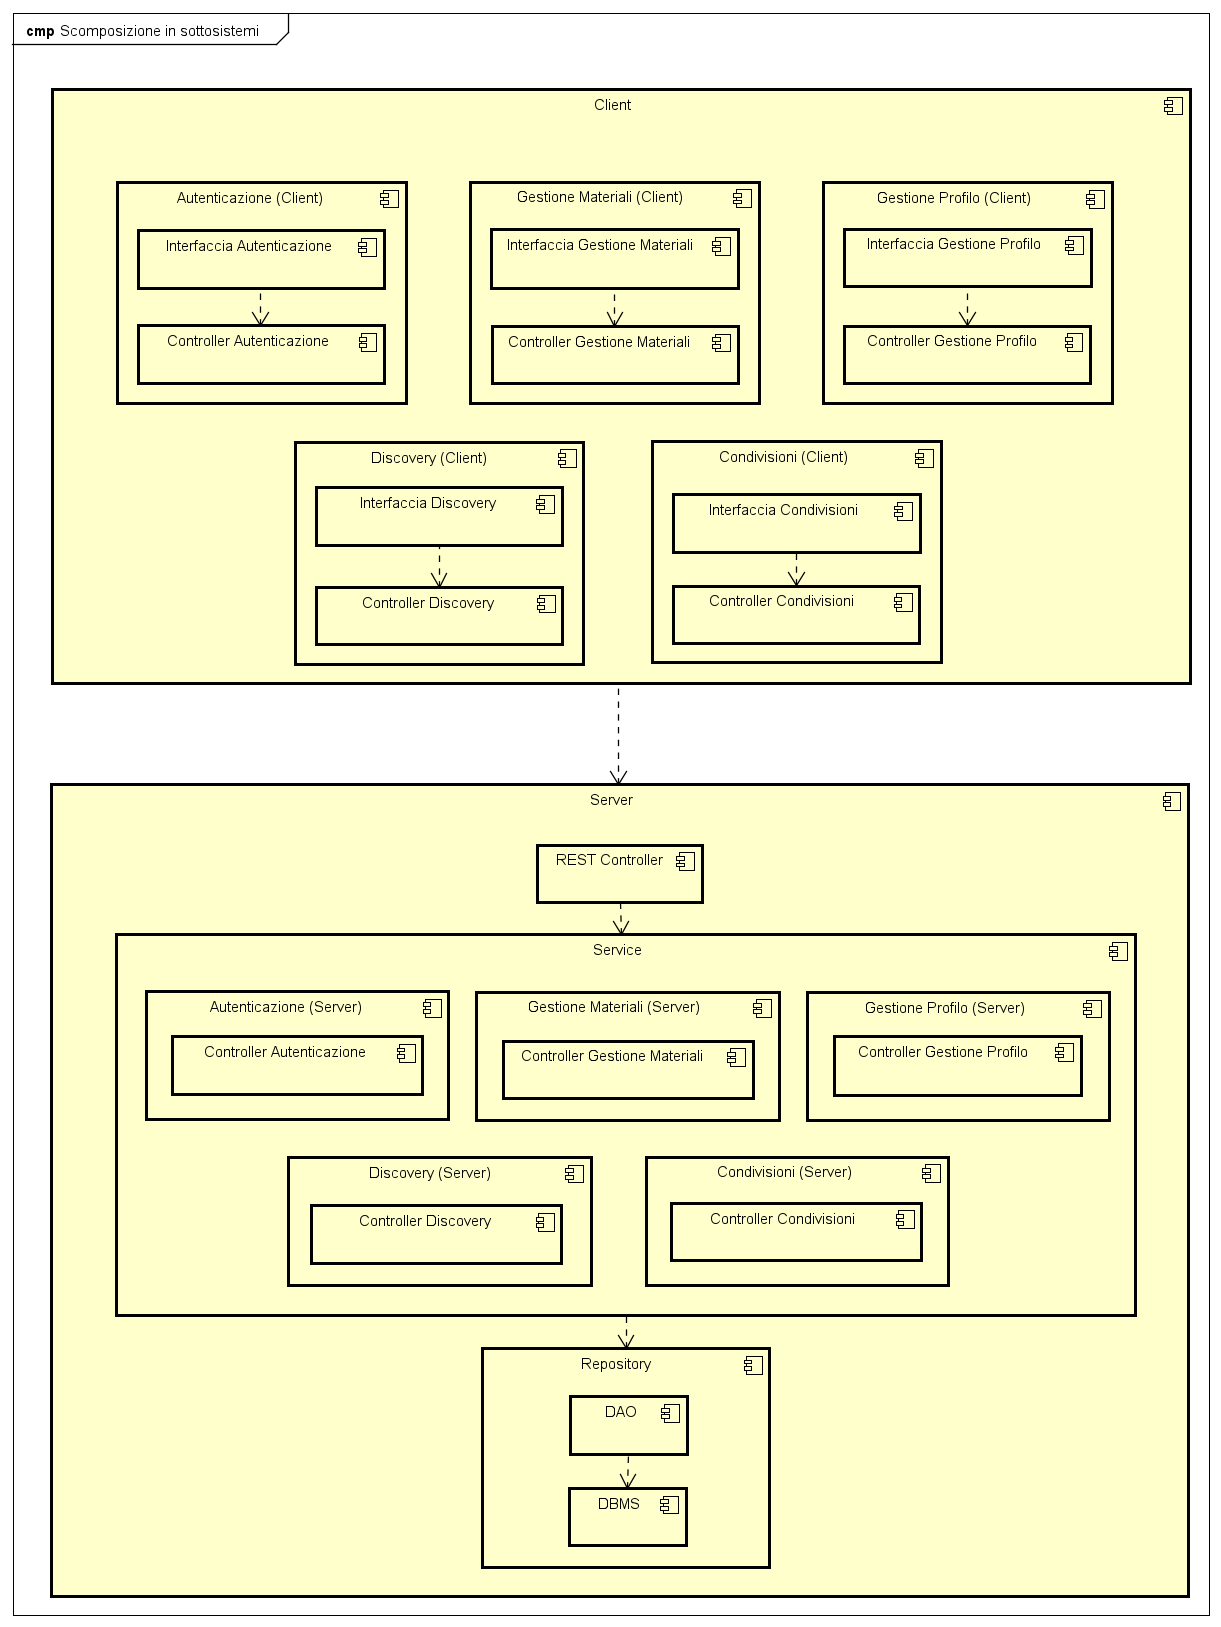
\includegraphics[width=0.95\textwidth, height=0.90\textheight, keepaspectratio]{Immagini/Scomposizione in sottosistemi.png}
    \caption{Scomposizione in sottosistemi}
\end{figure}

% \subsubsection{Gestione Autenticazione}
% Il sottosistema Gestione Autenticazione comprende i componenti che permettono lo svolgimento delle operazioni di login, registrazione e logout del Membro AFAM tramite credenziali, e autenticazione tramite identità digitale. Comprende inoltre i componenti adibiti a recupero e modifica password, e il componente relativo alla generazione del codice OTP.

% \subsubsection{Gestione Profilo}
% Il sottosistema Gestione Profilo comprende i componenti che permettono la visualizzazione e aggiornamento dei dati anagrafici e professionali, nonché la modifica dell'immagine di profilo, della visibilità del profilo e il calcolo della percentuale di completamento. Contiene inoltre il componente necessario per il collegamento dell'identità SPID.

% \subsubsection{Gestione Materiali}
% Il sottosistema Gestione Materiali comprende i componenti necessari al caricamento e gestione (CRUD) dei materiali, nonché le funzionalità di gestione degli ArtID, associazione di tag e stati di visibilità (Pubblico/Privato/Unlisted), gestione dei preferiti e anteprima dell'ArtID.



% \begin{itemize}
%     \item \textbf{Gestione Autenticazione:} login, registrazione e logout del Membro AFAM tramite credenziali, con rilascio di token JWT. Predisposti: autenticazione con identità digitale (SPID), verifica a due fattori tramite OTP, recupero e modifica password, eliminazione account.
%     \item \textbf{Gestione Profilo:} visualizzazione e aggiornamento dei dati anagrafici e professionali, immagine di profilo, impostazione del profilo come pubblico o privato e calcolo della percentuale di completamento. Predisposto: collegamento dell'identità SPID.
%     \item \textbf{Gestione Materiali:} caricamento e gestione (CRUD) dei materiali con persistenza del contenuto come BLOB, organizzazione in contenitori ArtID, associazione di tag e stati di visibilità (Pubblico/Privato/Unlisted), gestione dei preferiti e anteprima dell'ArtID.
%     \item \textbf{Gestione Condivisione:} condivisione interna verso altri Membri e condivisione esterna tramite link con scadenza e attivazione/disattivazione, con tracciamento degli accessi (contatore dei clic e data dell'ultimo accesso).
%     \item \textbf{Gestione Certificazioni:} caricamento, download e rimozione di attestati con metadati descrittivi e livello di visibilità.
%     \item \textbf{Discovery:} ricerca dei profili pubblici e dei contenuti per dati nominativi e per competenze/tag (predisposto).
% \end{itemize}

% \section{Architettura del Sistema e Panoramica dei Sottosistemi}


%----------------------------------------------------------------------------------------
%	1. AUTH SUBSYSTEM
%----------------------------------------------------------------------------------------
\subsubsection{Sottosistema di Autenticazione}
Questo sottosistema è responsabile della sicurezza, dell'identificazione e del controllo degli accessi di tutti gli utenti all'interno della piattaforma.

\begin{itemize}
    \item \textbf{Responsabilità Principali:}
    \begin{itemize}[noitemsep]
        \item Gestione del ciclo di vita delle sessioni utente (Login, Logout e Registrazione dei Membri).
        \item Integrazione con i gateway ufficiali SPID per la verifica certificata dell'identità digitale.
        \item Generazione, invio e validazione di codici OTP (\textit{One-Time Password}) per i meccanismi di autenticazione a due fattori.
        \item Coordinamento delle procedure di recupero o modifica delle credenziali di accesso.
        \item Gestione della procedura di chiusura e cancellazione definitiva dell'account in conformità con le normative vigenti sulla protezione dei dati.
    \end{itemize}
\end{itemize}

%----------------------------------------------------------------------------------------
%	2. PROFILE SUBSYSTEM
%----------------------------------------------------------------------------------------
\subsubsection{Sottosistema di Gestione Profilo}
Questo sottosistema gestisce il ciclo di vita dei dati anagrafici, di contatto e formativi del Membro AFAM. Si occupa inoltre della persistenza e della gestione dei Certificati caricati dall'utente. Gestisce inoltre le preferenze sulla privacy.

\begin{itemize}
    \item \textbf{Responsabilità Principali:}
    \begin{itemize}[noitemsep]
        \item Manutenzione e aggiornamento delle informazioni personali e di contatto.
        \item Amministrazione delle impostazioni di visibilità del profilo e delle preferenze sulla ricezione delle condivisioni.
        \item Gestione completa (caricamento, modifica, consultazione ed eliminazione) dei Certificati e dei relativi file scaricabili associati.
    \end{itemize}
\end{itemize}

%----------------------------------------------------------------------------------------
%	3. MATERIAL SUBSYSTEM
%----------------------------------------------------------------------------------------
\subsubsection{Sottosistema di Gestione Materiali}
Questo sottosistema fornisce i metodi per la costruzione e manutenzione del portfolio digitale del Membro AFAM, costituito dagli \textit{ArtID} e dai Materiali in essi contenuti. Controlla l'archiviazione logica dei Materiali e la loro gestione, nonché la gestione degli \textit{ArtID}.

\begin{itemize}
    \item \textbf{Responsabilità Principali:}
    \begin{itemize}[noitemsep]
        \item Coordinamento delle operazioni di upload, catalogazione, filtraggio e rimozione e aggiunta ai preferiti dei Materiali.
        \item Strutturazione dell'identità artistica tramite la creazione e configurazione degli \textit{ArtID}, inclusa l'associazione di metadati quali descrizione e immagine e l'assegnazione di Tag descrittivi e l'aggiunzione dei Materiali.
        \item Gestione dei livelli di visibilità dei singoli \textit{ArtID}.
    \end{itemize}
\end{itemize}

%----------------------------------------------------------------------------------------
%	4. SHARING SUBSYSTEM
%----------------------------------------------------------------------------------------
\subsubsection{Sottosistema di Condivisione}
Questo sottosistema gestisce la creazione e la gestione delle Condivisioni verso l'esterno o verso altri utenti della piattaforma, nonché la gestione delle relative notifiche (tramite email) di presa visualizzazione o ricevuta condivisione.

\begin{itemize}
    \item \textbf{Responsabilità Principali:}
    \begin{itemize}[noitemsep]
        \item Condivisione mirata degli \textit{ArtID} verso specifici Membri registrati attraverso Condivisioni Interne.
        \item Generazione di Condivisioni Esterne costituite da token temporanei e link da poter condividere con Guest, con possibilità di impostare descrizioni e date di scadenza.
        \item Tracciamento dei contatori di visualizzazione dei link esterni e supporto alla modifica, disattivazione o revoca dei permessi di accesso.
    \end{itemize}
\end{itemize}

%----------------------------------------------------------------------------------------
%	5. DISCOVERY SUBSYSTEM
%----------------------------------------------------------------------------------------
\subsubsection{Sottosistema di Discovery}
Questo sottosistema costituisce il motore di ricerca e consultazione pubblica della piattaforma, pensato per l'esplorazione rapida da parte di Guest. Espone i contenuti in modalità di sola lettura, applicando rigidi filtri di sicurezza per rispettare le impostazioni di privacy definite dai Membri.

\begin{itemize}
    \item \textbf{Responsabilità Principali:}
    \begin{itemize}[noitemsep]
        \item Fornitura di funzionalità di ricerca testuale (anche per corrispondenza parziale del nome) per l'individuazione dei Membri dando la possibilità di consultarne il Profilo o ArtID da questi creati.
        \item Controllo dei permessi di visualizzazione del Profilo o dei singoli ArtID, esponendo solamente quello che il Membro ha contrassegnato come Pubblico.
    \end{itemize}
\end{itemize}


\clearpage

\subsection{Mappatura degli oggetti nei sottosistemi}
Di seguito sono riportate le funzionalità offerte dai sottosistemi:

\subsubsection{Autenticazione}

\begin{figure}[H]
    \centering
    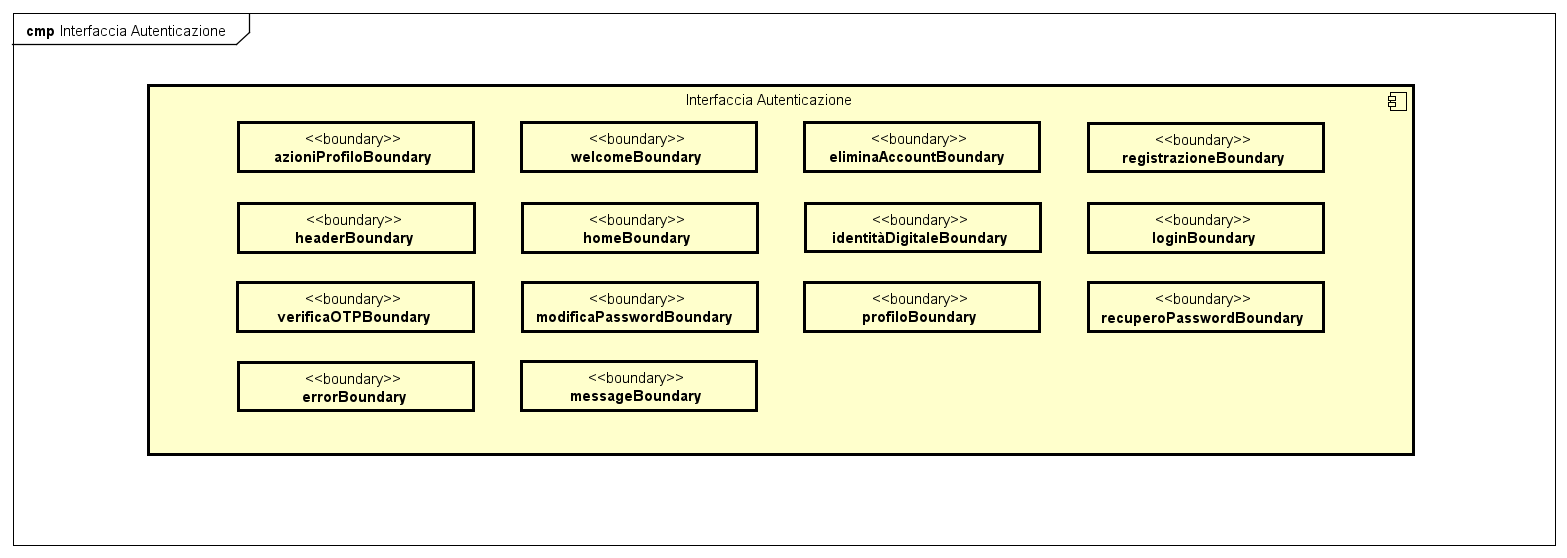
\includegraphics[width=0.95\textwidth, height=0.90\textheight, keepaspectratio]{Immagini/sottosistemi/Interfaccia Autenticazione.png}
\end{figure}

\begin{figure}[H]
    \centering
    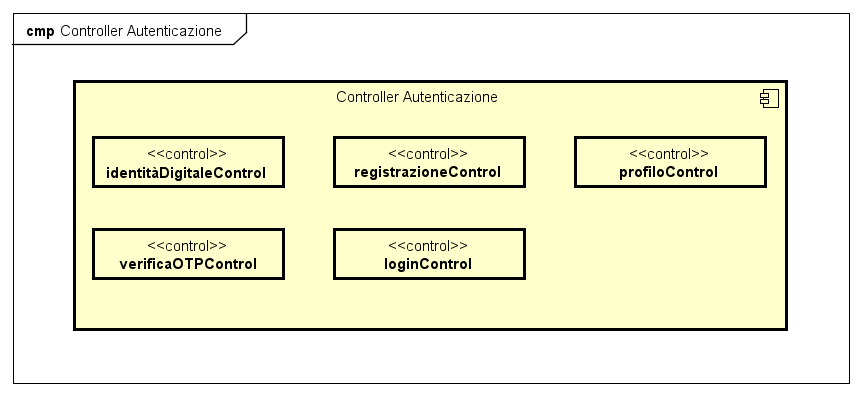
\includegraphics[width=0.95\textwidth, height=0.90\textheight, keepaspectratio]{Immagini/sottosistemi/Controller Autenticazione.png}
\end{figure}

\newpage

\subsubsection{Gestione Profilo}

\begin{figure}[H]
    \centering
    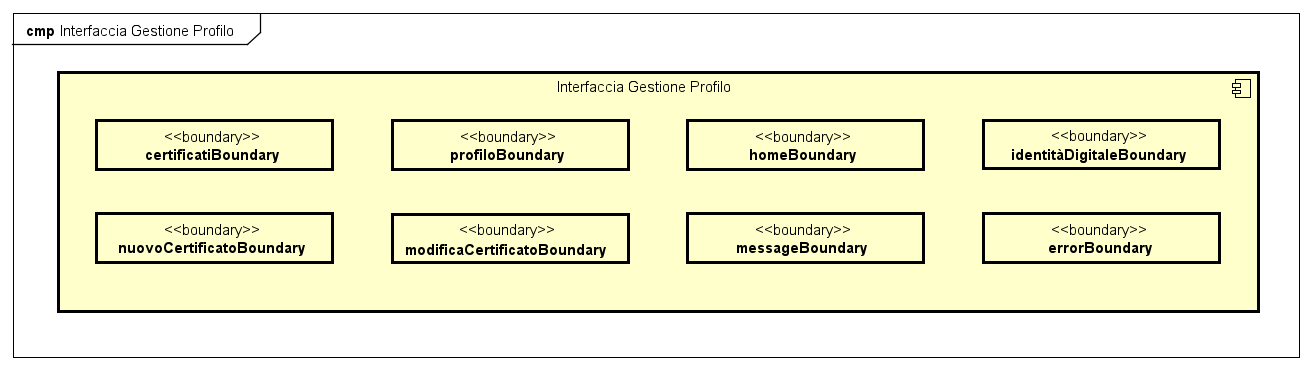
\includegraphics[width=0.95\textwidth, height=0.90\textheight, keepaspectratio]{Immagini/sottosistemi/Interfaccia Gestione Profilo.png}
\end{figure}

\begin{figure}[H]
    \centering
    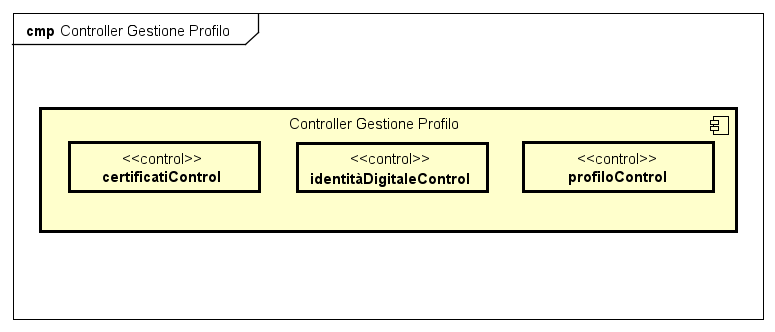
\includegraphics[width=0.95\textwidth, height=0.90\textheight, keepaspectratio]{Immagini/sottosistemi/Controller Gestione Profilo.png}
\end{figure}

\newpage

\subsubsection{Gestione Materiali}

\begin{figure}[H]
    \centering
    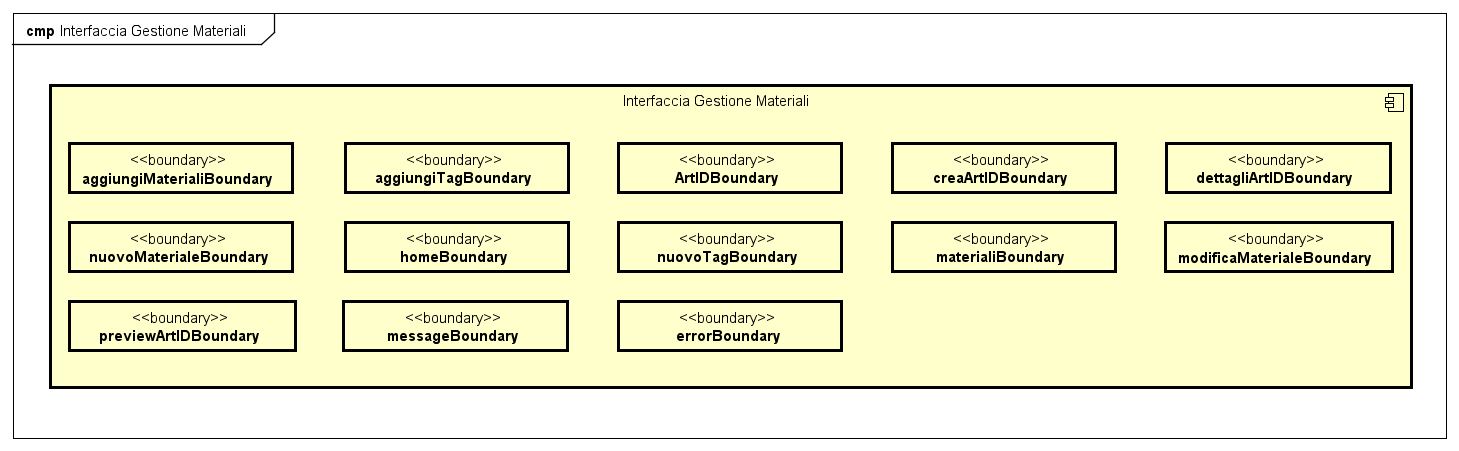
\includegraphics[width=0.95\textwidth, height=0.90\textheight, keepaspectratio]{Immagini/sottosistemi/Interfaccia Gestione Materiali.png}
\end{figure}

\begin{figure}[H]
    \centering
    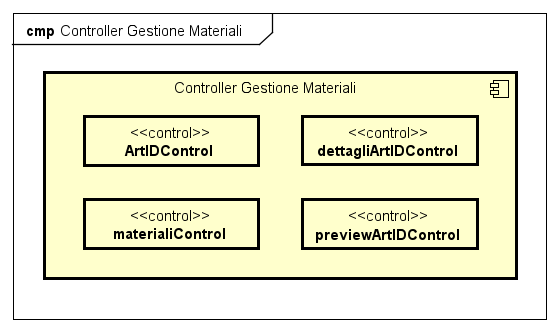
\includegraphics[width=0.95\textwidth, height=0.90\textheight, keepaspectratio]{Immagini/sottosistemi/Controller Gestione Materiali.png}
\end{figure}

\newpage

\subsubsection{Condivisione}

\begin{figure}[H]
    \centering
    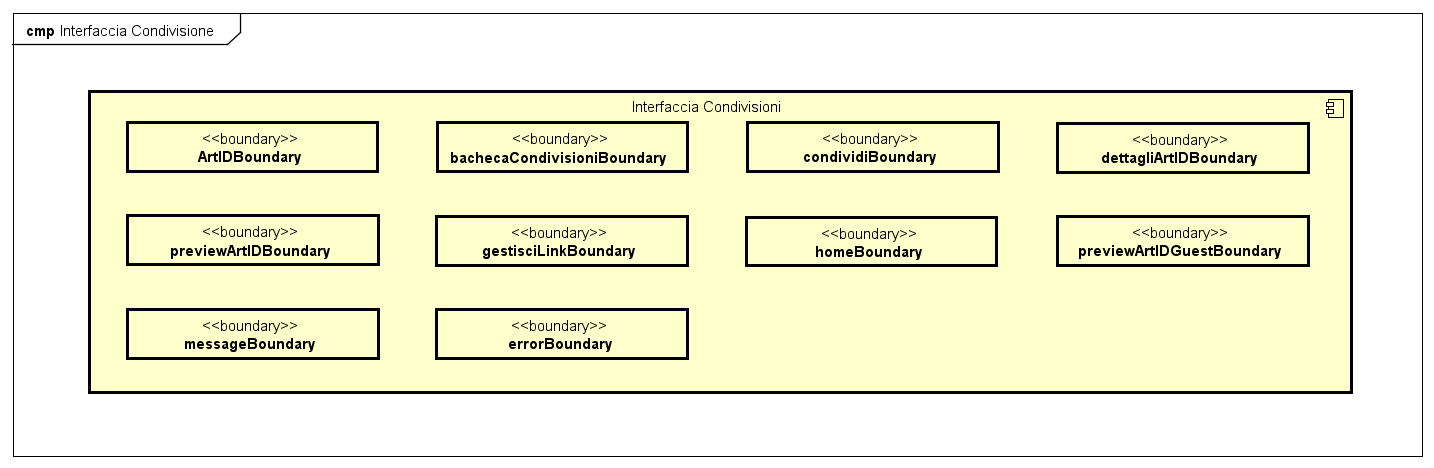
\includegraphics[width=0.95\textwidth, height=0.90\textheight, keepaspectratio]{Immagini/sottosistemi/Interfaccia Condivisione.png}
\end{figure}

\begin{figure}[H]
    \centering
    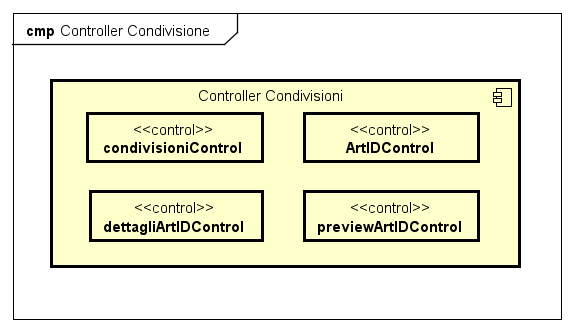
\includegraphics[width=0.95\textwidth, height=0.90\textheight, keepaspectratio]{Immagini/sottosistemi/Controller Condivisione.png}
\end{figure}

\newpage

\subsubsection{Discovery}

\begin{figure}[H]
    \centering
    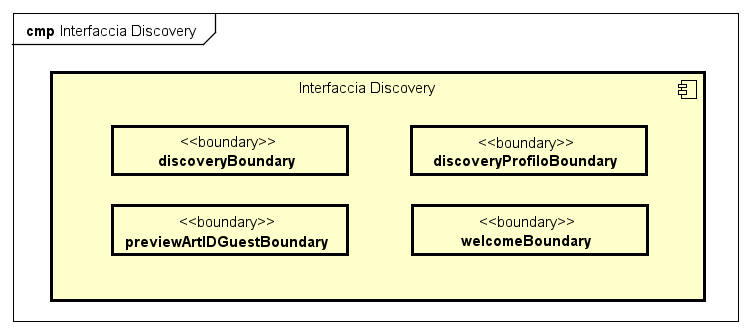
\includegraphics[width=0.95\textwidth, height=0.90\textheight, keepaspectratio]{Immagini/sottosistemi/Interfaccia Discovery.png}
\end{figure}

\begin{figure}[H]
    \centering
    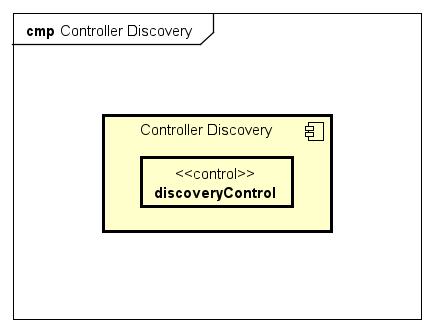
\includegraphics[width=0.95\textwidth, height=0.90\textheight, keepaspectratio]{Immagini/sottosistemi/Controller Discovery.png}
\end{figure}

\newpage

\subsection{Mappatura Hardware/Software}

La mappatura dei componenti software sui nodi hardware del sistema riflette la separazione strutturale introdotta dallo stile Client-Server e dal pattern MVC. Il sistema è distribuito su due macro-nodi principali:

\begin{itemize}
    \item \textbf{Nodo ``Dispositivo Utente'' (Client):} Ospita il sottosistema \textit{View} e le componenti di interfaccia del \textit{Controller}. Questo nodo hardware (rappresentato dai dispositivi personali degli utenti) esegue l'applicazione client, gestendo l'interazione diretta con l'utente e l'invio delle richieste verso il server centralizzato.
    \item \textbf{Nodo Centralizzato ``Server AFAM'':} Rappresenta il nucleo del sistema e ospita la logica di business principale (\textit{Controller} di backend), l'architettura \textit{Repository} e il \textit{DBMS}. Questo nodo gestisce la sicurezza, la persistenza transazionale dei dati all'interno della sorgente dati e l'elaborazione dei portfolio multimediali, esponendo le API necessarie per permettere ai nodi client di comunicare e recuperare o inserire informazioni in modo sicuro.
\end{itemize}

Le comunicazioni tra il nodo client e il server centrale avvengono tramite canali di rete protetti, isolando completamente l'accesso diretto al DBMS dall'ambiente esterno a garanzia della sicurezza dei dati istituzionali.

\begin{figure}[H]
    \centering
    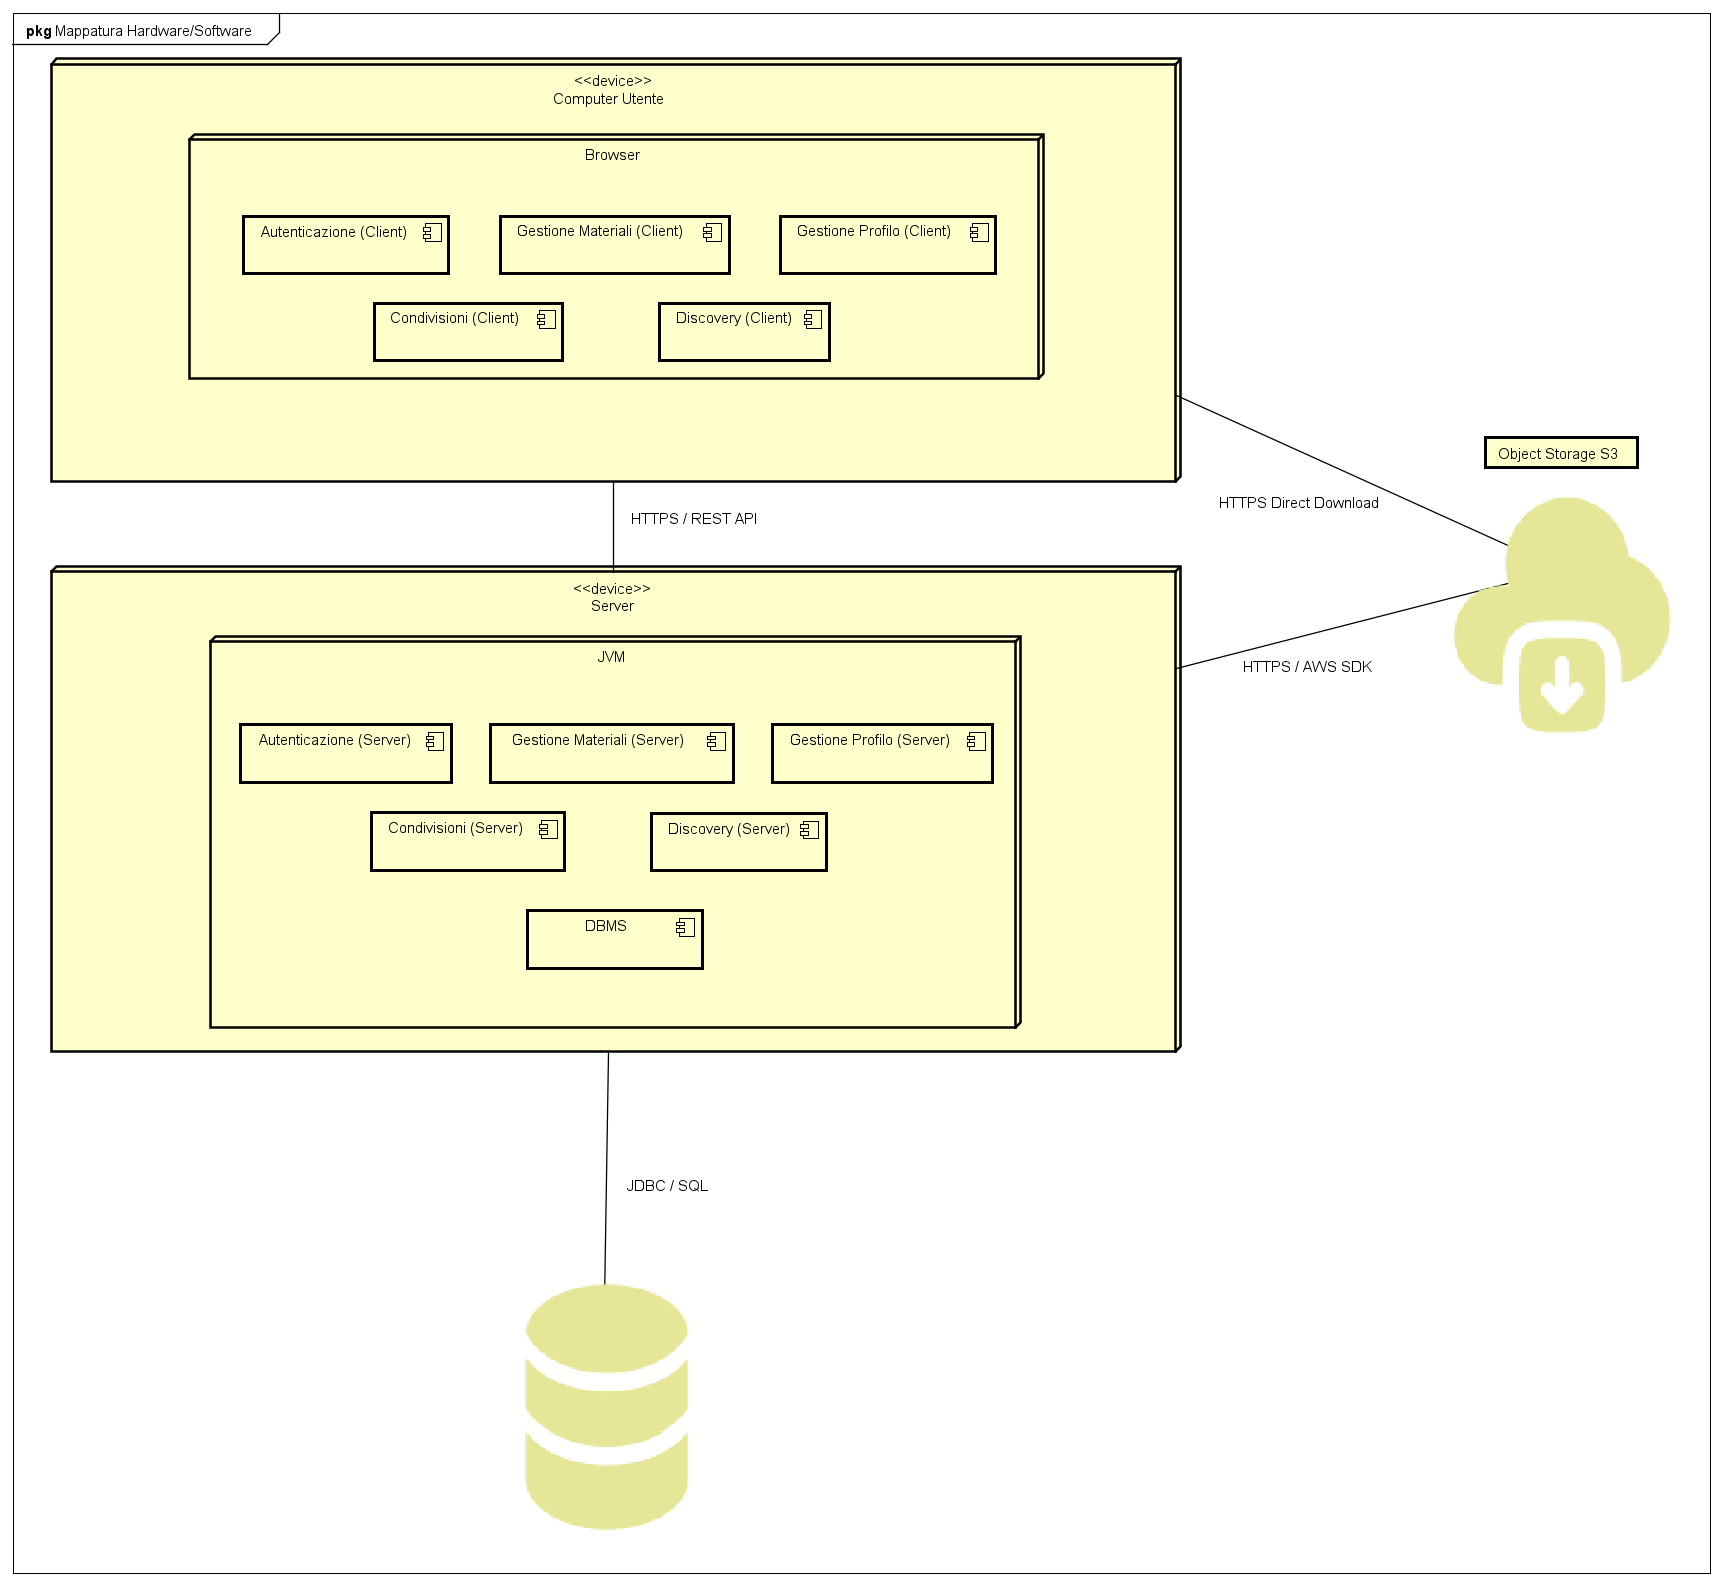
\includegraphics[width=0.95\textwidth, height=0.90\textheight, keepaspectratio]{Immagini/Mappatura Hardware_Software.png}
    \caption{Mappatura Hardware/Software}
\end{figure}
